\documentclass{article}
\usepackage{graphicx}
\usepackage{listings,xcolor}
\lstset{
    string=[s]{"}{"},
    stringstyle=\color{blue},
    comment=[l]{:},
    commentstyle=\color{black},
    breaklines=true,
}
\begin{document}

\title{Assignment 2}
\author{Joshua Graham}

\maketitle
\pagebreak
\begin{abstract}
All Scripts used in the assignment can be found in the A2 folder, if needed.

\end{abstract}

\section{Problem 1}
	The first question, generating 1000 links, was only hard at first because I tried to cut corners. I actually had to generate links twice, due to the fact that the first time I generated them I decided to use verify=false in my requests object. Instead of throwing links out that returned with a permission error, I ignored the error and kept them. After changing that back, I threw out anything with an error I could not deal with, and regenerated the links.

Beyond that, one of the issues I ran into, was when given a link from google, sometimes it would not redirect with the redirect=True flag enabled. As far as I can tell I weeded most of them out, but there are probably a few left in the list.

It is important to note that I generated slightly above 1000 links. I'm not entirely sure why my program stopped at 1052, but I decided to leave all the links in there regardless. I felt that chooseing 52 links by hand to throw out would be micromanging the data too much. For a class, it probably wouldn't have been an issue, I'm just not sure the morality of choosing which data to post, so I left the extra 52 in.

The links can be found in the A2/ directory, under the file links.txt.
\pagebreak
\section{Question 2}


Below is the graph for the number of sites vs the number of mementos.
\begin{center}
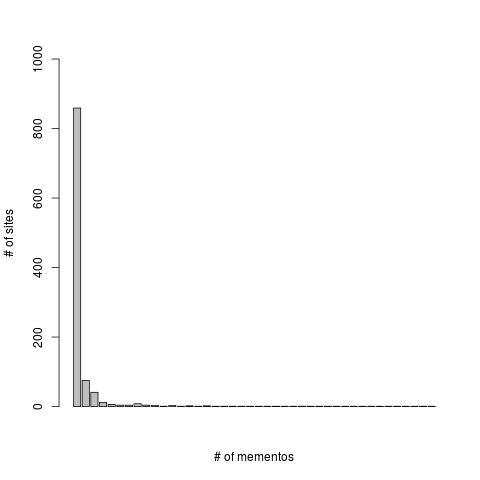
\includegraphics[scale=0.6]{images/plot1.jpeg}
\end{center}

My only complaint with the graph is that I cannot get the bottom axis to show up. I can tell, through trial and error, that it goes up by one each iteration to the right. It is also missing a few far outside of the scope of the bars. I have one link with over 80,000 memetos, and it isn't shown. Anything outside of the range of the graph only has 1 site with that many mementos. 

This is roughly when I regnereated the links, as I felt the results were skewed due to links the process could not follow. Below is data1023.json. It is the 1023rd link in the list. The rest can be found in the directory A2/Mementos/. This one wasn't as hard, and in the long run, was the least time consuming of the three questions. The only part that troubled me was not throwing out links that 404'd. After I asked on Slack, and started assuming links that 404 had 0 mementos, the question was easy again.
\begin{lstlisting}
{
  "mementos": {
    "first": {
      "datetime": "2018-02-10T04:22:43Z",
      "uri": "http://web.archive.org/web/20180210042243/http://www.uppermichiganssource.com/content/news/Dome-Softball-Tournament-raising-money-for-Area-36-Special-Olympics--473640333.html"
    },
    "list": [
      {
        "datetime": "2018-02-10T04:22:43Z",
        "uri": "http://web.archive.org/web/20180210042243/http://www.uppermichiganssource.com/content/news/Dome-Softball-Tournament-raising-money-for-Area-36-Special-Olympics--473640333.html"
      }
    ],
    "last": {
      "datetime": "2018-02-10T04:22:43Z",
      "uri": "http://web.archive.org/web/20180210042243/http://www.uppermichiganssource.com/content/news/Dome-Softball-Tournament-raising-money-for-Area-36-Special-Olympics--473640333.html"
    }
  },
  "timegate_uri": "https://memgator.cs.odu.edu/timegate/http://www.uppermichiganssource.com/content/news/Dome-Softball-Tournament-raising-money-for-Area-36-Special-Olympics--473640333.html%0A",
  "timemap_uri": {
    "link_format": "https://memgator.cs.odu.edu/timemap/link/http://www.uppermichiganssource.com/content/news/Dome-Softball-Tournament-raising-money-for-Area-36-Special-Olympics--473640333.html%0A",
    "cdxj_format": "https://memgator.cs.odu.edu/timemap/cdxj/http://www.uppermichiganssource.com/content/news/Dome-Softball-Tournament-raising-money-for-Area-36-Special-Olympics--473640333.html%0A",
    "json_format": "https://memgator.cs.odu.edu/timemap/json/http://www.uppermichiganssource.com/content/news/Dome-Softball-Tournament-raising-money-for-Area-36-Special-Olympics--473640333.html%0A"
  },
  "original_uri": "http://www.uppermichiganssource.com/content/news/Dome-Softball-Tournament-raising-money-for-Area-36-Special-Olympics--473640333.html%0A",
  "self": "https://memgator.cs.odu.edu/timemap/json/http://www.uppermichiganssource.com/content/news/Dome-Softball-Tournament-raising-money-for-Area-36-Special-Olympics--473640333.html%0A"
}
\end{lstlisting}
\pagebreak
\section{Question 3}

Below is the scatterplot for this question. I ran out of time, or I'd make sure the scatterplot looked better. However, it does correctly represent the information I generated.
\begin{center}
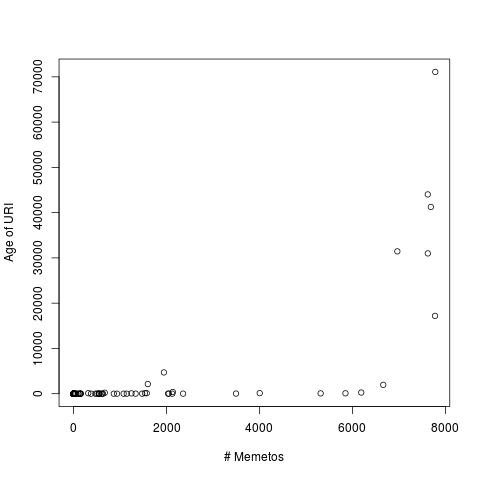
\includegraphics[scale=0.6]{images/plot2.jpeg}
\end{center}

Where question 2 was the shortest question, question 3 was the easiest. I downloaded and installed docker, after which I had a choice. I could attempt to integreate it with python. Or I could use bash. I chose bash. Below is the one-liner I used to iterate through the file and run the carbon date process on each of the links.
\begin{lstlisting}[language=bash]
hold=0; for line in $(cat links.txt); do hold=$((hold+1)); echo -n $hold; echo ": $line"; sudo docker run --rm -it oduwsdl/carbondate ./main.py -l search $line > "$hold.json"; done
\end{lstlisting}

To break it down, I looped through each line in the links.txt, incrementing hold each time, setting the current links to line. I ran docker as the super user on the line variable, then saved the output to the current number represented by hold, followed by the json extension. This, however, even on my home machine, took hours. I set it going at 10pm and it finished at 8am. I'm glad I didn't wait until the last day to do this.

I could not get the docker deamon to work correctly on my system without running as the super user. I'll have this fixed by the next assignment, I just need time to sit down and fix it. Below is 528.json, the rest can be found in the CarbonDateJson/ directory.
\begin{lstlisting}
{
  "self": "",
  "uri": "https://mic.com/articles/187743/2018-winter-olympics-puerto-rico-skier-charles-flaherty-breaks-the-territorys-20-year-dry-spell",
  "estimated-creation-date": "2018-02-08T17:17:53",
  "earliest-sources": [
    "twitter.com"
  ],
  "sources": {
    "bing.com": {
      "earliest": ""
    },
    "twitter.com": {
      "earliest": "2018-02-08T17:17:53"
    },
    "backlinks": {
      "earliest": ""
    },
    "pubdate": {
      "earliest": ""
    },
    "bitly.com": {
      "earliest": ""
    },
    "google.com": {
      "earliest": ""
    },
    "last-modified": {
      "earliest": ""
    }
  }
}
\end{lstlisting}
\end{document}